\documentclass{book}

\usepackage[english]{babel}
\usepackage[utf8]{inputenc}

\usepackage{tikz}
\usetikzlibrary{calc}

\usepackage{amsfonts}
\usepackage{amsmath}
\usepackage{amsthm}

\newcommand*\V[1]{ \boldsymbol{#1}}

\title{Simulation of plasma with \texttt{cpic} using OmpSs}
\author{Rodrigo Arias Mallo}
\date{\today}

\begin{document}

\maketitle
\tableofcontents

\chapter{Introduction}

It may be surprising to find out that the most common state of matter is plasma 
when we look at the universe. A plasma is a gas in which at least one electron 
of the atom is separated, so it remains positively charged (ionized) 
\cite{chen}.  Usually this happens in the vacuum

\chapter{Plasma simulation}



\section{1D electrostatic simulation}
The magnetic field is ignored.

\section{2D simulation}
The magnetic field is not ignored.

\section{Electromagnetism}

\subsection{Background magnetic field}

To introduce the magnetic field, the equations are:

$$ $$

\subsection{Boris integrator} % Integrator?

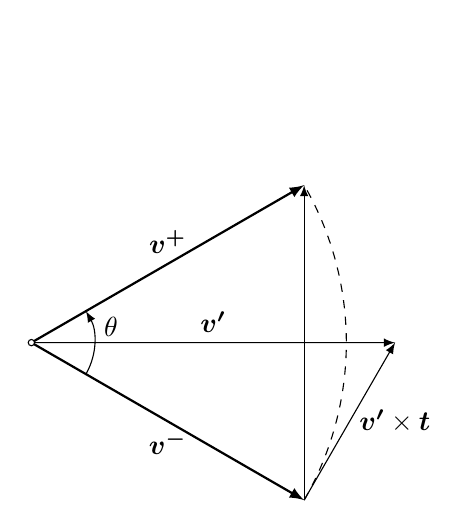
\begin{tikzpicture}[
	scale=2,
	>=latex,
	migrid/.style ={step=0.5,color=red!50!white, very thin},
	micurva/.style ={thick, color=blue},
	mipunto/.style ={color=gray}]

	\def\centerarc[#1](#2)(#3:#4:#5)% Syntax: [draw options] (center) (initial angle:final angle:radius)
		{\draw[#1] ($(#2)+({#5*cos(#3)},{#5*sin(#3)})$) arc (#3:#4:#5); }

	\def\startangle{-30}
	\def\midangle{0}
	\def\endangle{30}
	\def\radius{2.0}
	\pgfmathsetmacro{\vlen}{\radius*tan(\startangle)}%

	\coordinate (O) at (0,0);
	\coordinate (S) at (\startangle:\radius);
	\coordinate (E) at (\endangle:\radius);

	\centerarc[dashed](O)(\startangle:\endangle:\radius);
	\centerarc[->](O)(\startangle:\endangle:0.2*\radius);

	\draw (O)+(0.4,0.1) node [right] {$\theta$};

	\draw [thick,->] (O) -- (E) node [midway, above] {$\V{v^+}$};
	\draw [thick,->] (O) -- (S) node [midway, below] {$\V{v^-}$};

	\path (S) +(\startangle-90:\vlen) coordinate (V1E);
	\path (E) +(\endangle-90:\vlen) coordinate (V3E);

	%\draw [->] (E) -- (V3E);
	\draw [->] (S) -- (V1E) node [midway, right] {$\V{v'} \times \V t$};

	\draw [->] (O) -- (V1E) node [midway, above] {$\V{v'}$};
	\draw [->] (S) -- (E);

	\draw [fill=white] (O) circle (0.02);

\end{tikzpicture}

$$ \V{v^-} $$
$$ \V s = \frac{2 \V t}{1 + \V t^2} $$
$$ \V{v^+} = \V{v^-} + \V{v}' \times \V{s} $$

\chapter{Parallelization}

\section{Data structures}

\chapter{Results}

\chapter{Conclusions}

\bibliographystyle{siam}
\bibliography{bib}

\end{document}
